\subsection{Variance reduction}
\subsubsection{Cell-based biasing}
\label{sec:vr:cell}

Cell-based weight window can be generated with the following arguments:

\lstinputlisting[language=bash,numbers=none,backgroundcolor=\color{yellow!20},frame=tb]{UserGuide/cell-biasing.sh}

\begin{description}
\item[-w] should precede all weight-related arguments.
\item[--weightEnergyType] defines energy grid. With the {\tt wwg} card you can either use this expression or {\tt --wwgE}.
  If use use the word ``energy'' then the format is energy (below \SI{0.1}{\mega\electronvolt}) followed by default weight for that bin (0.95) etc.
  If you drop the word ``energy'' then you just set the energy grid.
  In the given example for energies below  the default weight is 0.95 etc.
  Alternatively you can use pre-defined keywords:
  {\tt basic}, {\tt high}, {\tt mid} and {\tt flat}\footnote{Energy-weight binnings for these keywords are defined in \tt{System/weights/WeightControl.cxx}}.
\item[--weightSource] This argument defines points in space. We can define as many as we want, but only those used with {\tt weightObject} will be used.
\item[--weightPlane] This argument defines planes. We can define as many as we want, but only those used with {\tt weightObject} will be used.
\item[--weightObject] {\tt BBunkerWallMainWall1 TP1 1.0 0.15 1e-20 }: object we are interested in calculating; {\tt TP1}: tally plane 1;
  \mbox{\tt 1.0 1.0 0.15 1e-20}: energy above \SI{1}{\mega\electronvolt} (below it we are not interested~--- use default values);
  {\tt 1.0}: scale factor; 
  {\tt 0.15}: density factor; {\tt 1e-20}: minimum weight % 41:12
\item[--voidUnMask] By default (without this argument) the importance of the surrounding void cell is zero. This argument sets it to one.
  It can be useful if we believe that particles travelling through the void cell can contribute into the tally.

\item[--weightObject] 
$\underset{
  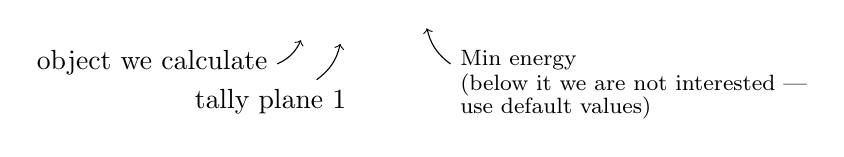
\begin{tikzpicture}
    \node[below left] at (-1,0) {object we calculate};  \draw[->](-1.0, -0.3) to[bend right=20] ++(0.3,2ex);
    \node[below left] at (0,-0.5) {tally plane 1};      \draw[->](-0.5, -0.5) to[bend right=20] ++(0.3,3ex);
    \node[below right] at (1.2,0.0) {\footnotesize{Min energy}};      \draw[->](1.2, -0.3) to[bend left=20] ++(-0.3,3ex);
    \node[below right] at (1.2,-0.3) {\footnotesize{(below it we are not interested~---}};
    \node[below right] at (1.2,-0.6) {\footnotesize{use default values)}};
  \end{tikzpicture}
}{\text{BBunkerWallMainWall1 TP1 1.0 0.15 1e-20}}$

\end{description}


\begin{landscape}
\begin{figure}
  \centering
  \subfloat[Horizontal view: geometry]{
    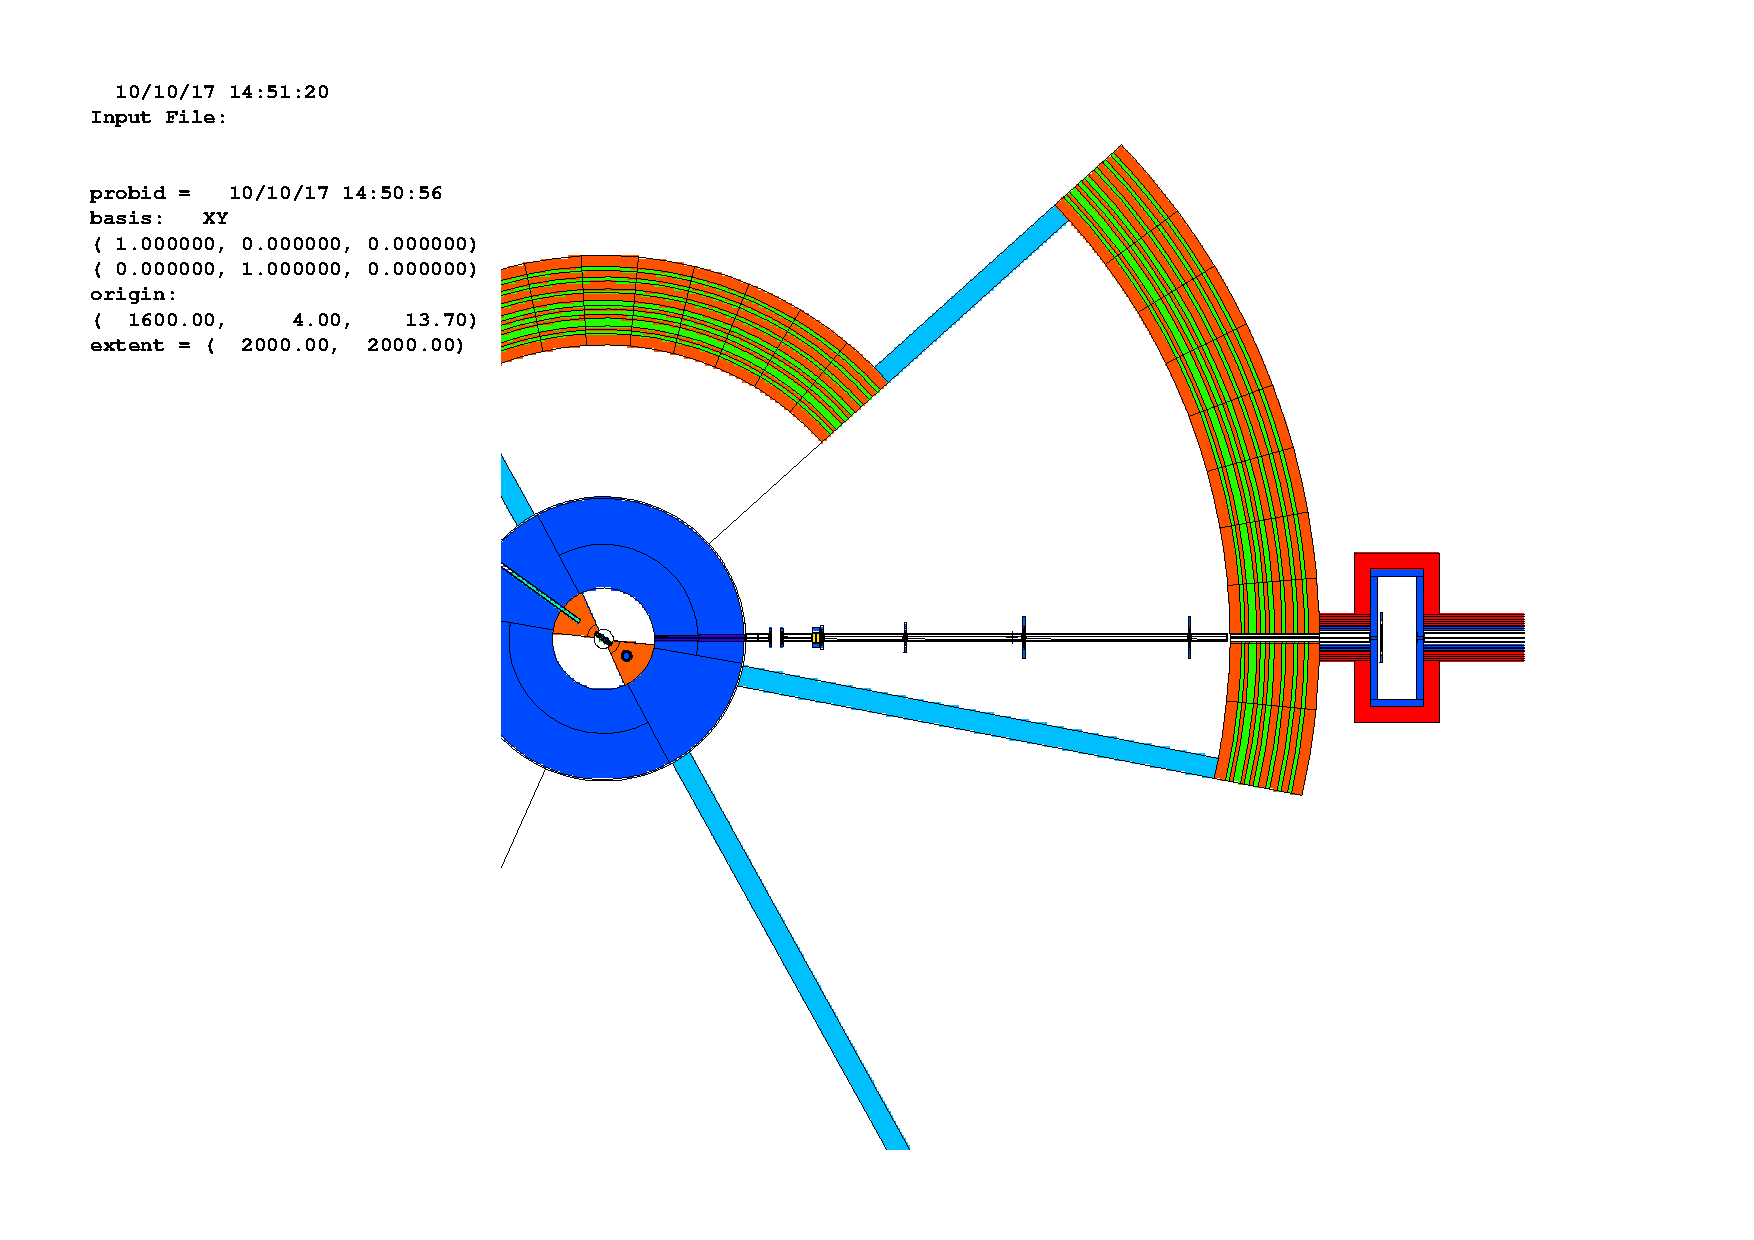
\includegraphics[width=0.5\linewidth,page=1,clip=true, trim=10cm 8cm 4cm 7cm]{UserGuide/cell-biasing.pdf}
  }
  \subfloat[Horizontal view: wwn]{
    \includegraphics[width=0.5\linewidth,page=3,clip=true, trim=10cm 8cm 4cm 7cm]{UserGuide/cell-biasing.pdf}
  } \\
  \subfloat[Vertical view: geometry]{
    \includegraphics[width=0.5\linewidth,page=2,clip=true, trim=10cm 8cm 4cm 7cm]{UserGuide/cell-biasing.pdf}
  }
  \subfloat[Vertical view: wwn]{
    \includegraphics[width=0.5\linewidth,page=4,clip=true, trim=10cm 8cm 4cm 7cm]{UserGuide/cell-biasing.pdf}
  }
  \caption{Cell-based weight window}
  \label{fig:vr:cell}
\end{figure}
\end{landscape}